\chapter{Caso de uso: \#BLM}
\label{chap:casouso}

Para mostrar el funcionamiento de la aplicación, a lo largo de este capítulo se desarrollará un caso de uso real y se irá
comentando paso a paso.

\section{Puesta en marcha del sistema}
\label{sec:casouso_puesta_en_marcha}

Como se mencionó en la Sección \ref{sec:herramientas_soporte}, para poder ejecutar la aplicación simplemente es necesario tener
instalado Docker y Docker-Compose. Una vez instalados, es necesario ejecutar el siguiente comando en la raíz del
proyecto:

\bigskip
\begin{Verbatim}
docker-compose up
\end{Verbatim}

\bigskip
A partir de este momento, Docker se encargará de descargar las imágenes necesarias para poner en marcha el sistema y de levantar los
contenedores. Una vez finalizado el proceso, se podrá acceder a la aplicación de forma local en la URL: \url{http://localhost:3000}.

\section{\textit{Dataset} del movimiento BLM}
\label{sec:casouso_dataset}

Como se comentó en el Capítulo \ref{chap:introduccion}, en las redes sociales se genera una gran cantidad de información y se debate sobre
diversos temas. Por ello, numerosos investigadores han utilizado esta información para crear lo que se conoce como "archivos sociales"
(Pybus et al., 2015 \cite{pybus2015hacking}; Acker et al., 2014 \cite{acker2014death}; Ruiz et al., 2020 \cite{ruiz2020cuentalo}),
que buscan preservar determinados aspectos de la interacción en las redes sociales y servir como base para futuras investigaciones
y estudios.

\bigskip
En este contexto, los tutores de este trabajo, utilizando una metodología propia para la creación de colecciones de referencia
a modo de archivos sociales
(Otero et al., 2021) \cite{oterorodilla2021}, han elaborado un \textit{dataset} sobre el fenómeno social
que se produjo tras la muerte de George Floyd en mayo de 2020 conocido como \textit{Black Lives Matter},
que implicó protestas en todo el mundo en las que se denunciaba la brutalidad policial y el racismo sistémico en Estados Unidos. Esta colección, 
disponible tanto en español como en inglés, recoge más de 260.000 posts referentes a más de 90.000 usuarios de la red social Reddit que compartieron contenido sobre este
fenómeno en el periodo de aproximadamente un año.

\bigskip
Sin embargo, debido a que la colección estaba formada por varios archivos diferentes en formato XML, donde unos contenían información de los hilos
de conversación en Reddit y otros posts de los usuarios que interactuaban en dichos hilos, fue necesario procesarlos y unificarlos
en un \textit{dataset} con un formato sencillo y aceptado por la aplicación. Así, se generaron tres \textit{datasets}, todos ellos
en inglés, en formato NDJSON, cada uno con 
un número diferente de posts para cada usuario (50, 500 y 1000) con el fin de analizar las posibles diferencias en cuanto a los resultados
obtenidos por el perfilado. Además, destacar que, ya que ninguno de estos tres \textit{datasets} están etiquetados, no conocemos a priori 
la distribución de cada característica y por lo tanto no podemos obtener una medida del balanceo entre las clases.

\section{Subida del \textit{dataset}}
\label{sec:casouso_subida_dataset}

Una vez contamos con el \textit{dataset} que vamos a procesar para el perfilado, el primer paso es subirlo a la aplicación. Para ello,
en la página de inicio, mostrada en la Figura \ref{fig:casouso_home}, se puede observar, a mayores de un
campo de búsqueda por usuario de Twitter, un campo para la subida del \textit{dataset}, que será el que empleemos.
Destacar que, en este caso y a lo largo del resto de secciones de este capítulo,
se mostrarán las capturas de pantalla tanto de la versión de escritorio (izquierda) como de la versión móvil (derecha).

\bigskip
\begin{figure}[H]
	\centering
	\begin{subfigure}[c]{0.74\textwidth}
			\centering
			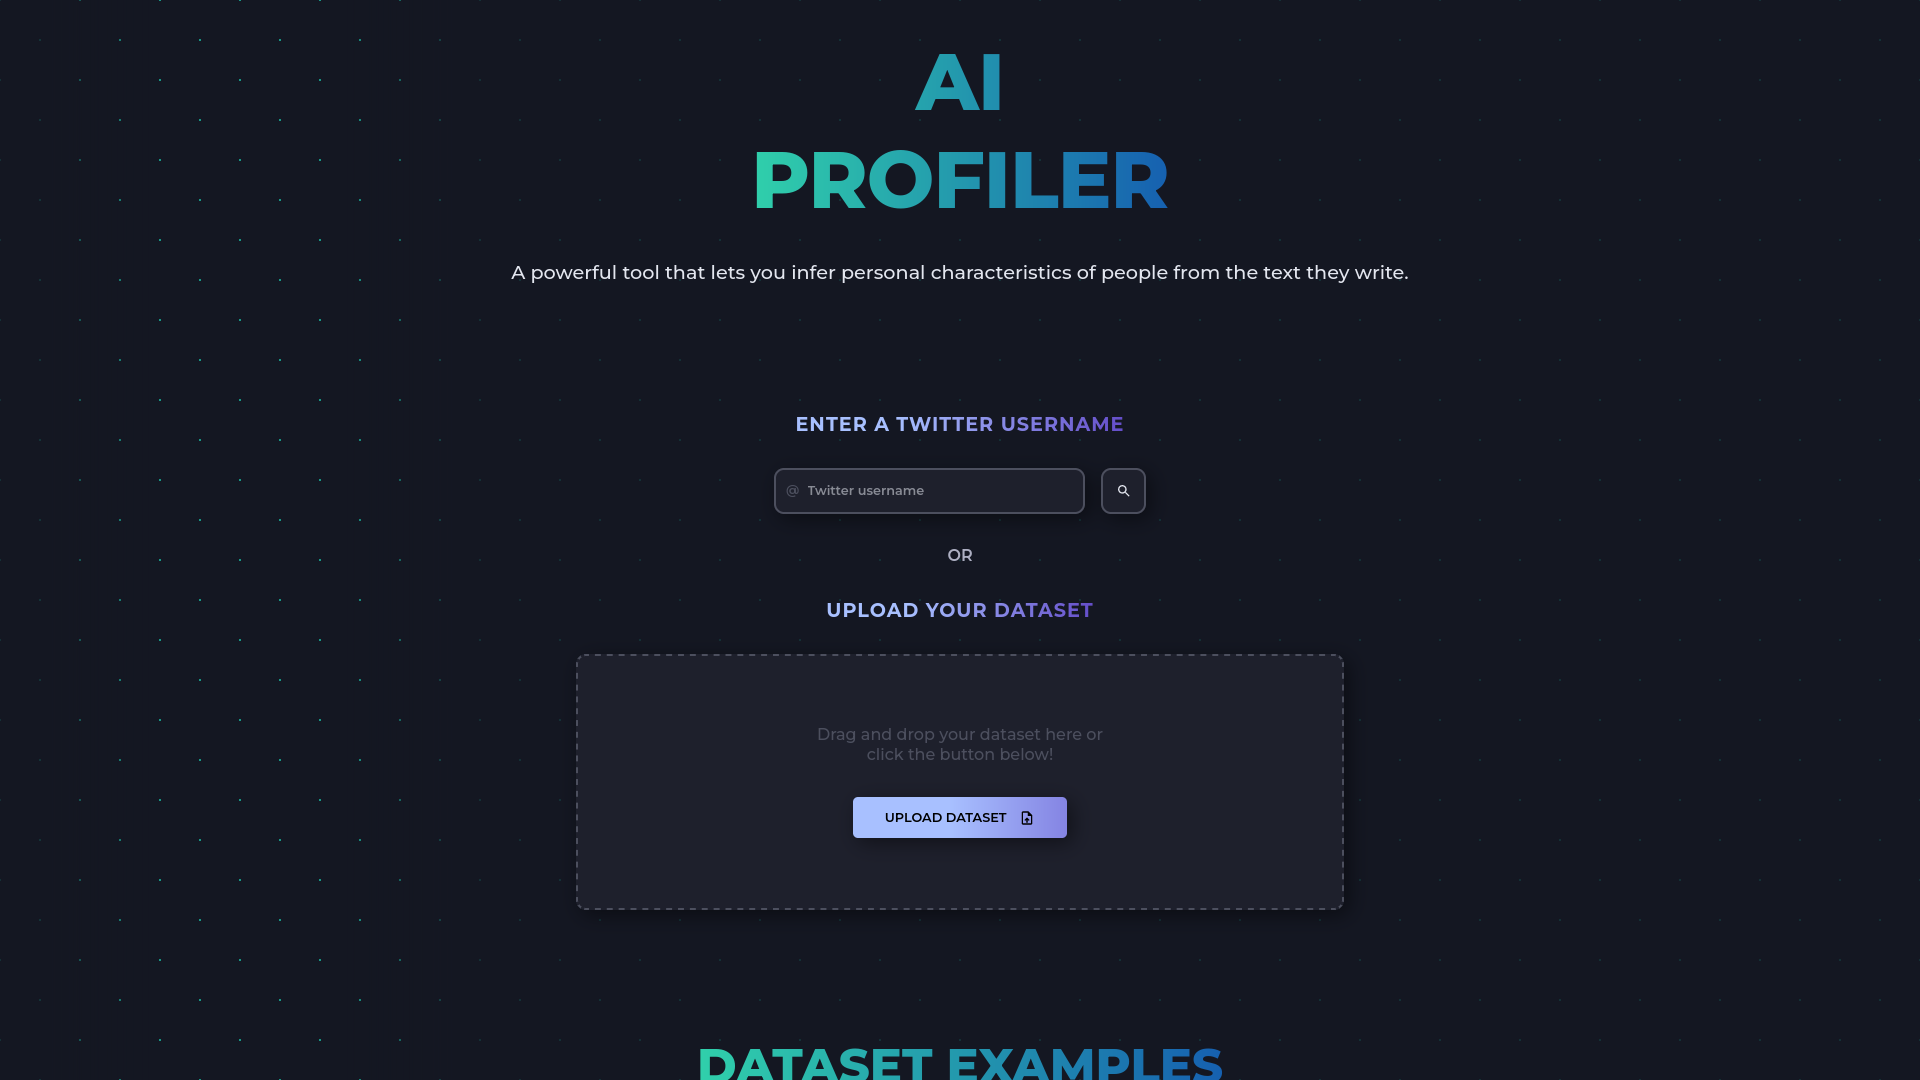
\includegraphics[width=\textwidth]{imagenes/home.png}
			\label{fig:casouso_home_escritorio}
	\end{subfigure}
	\hfill
	\begin{subfigure}[c]{0.21\textwidth}
			\centering
			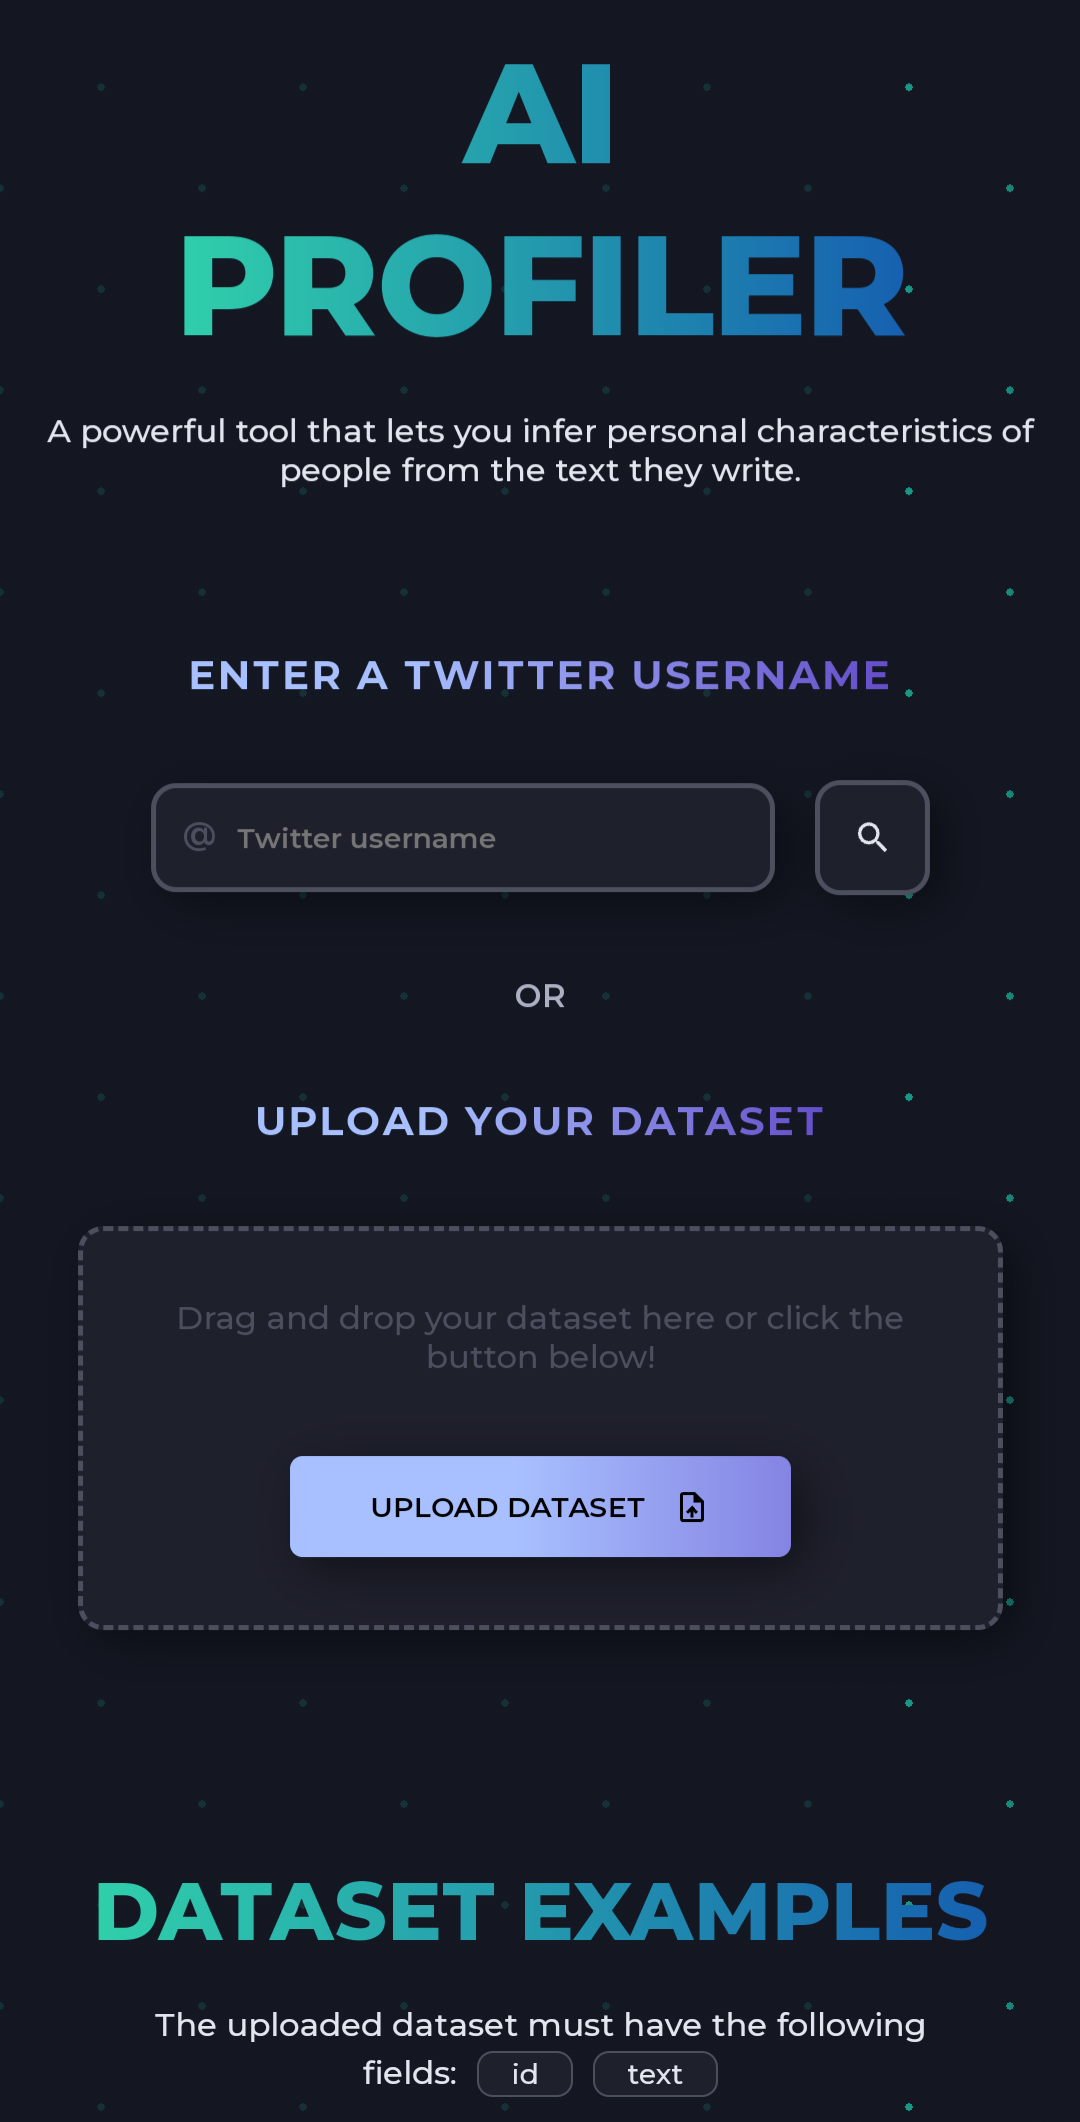
\includegraphics[width=\textwidth]{imagenes/home_movil.png}
			\label{fig:casouso_home_movil}
	\end{subfigure}
	\vspace{-1\baselineskip}
	\caption{Página de inicio de la aplicación}
	\label{fig:casouso_home}
\end{figure}

\bigskip
Asimismo, si el usuario desea conocer cual es la estructura y los campos que debe contener el \textit{dataset} que va a subir,
puede hacerlo consultando la sección de ejemplos, mostrada en la Figura \ref{fig:casouso_examples}, visible tras hacer \textit{scroll}
en la misma página de inicio.

\bigskip
\begin{figure}[H]
	\centering
	\begin{subfigure}[c]{0.74\textwidth}
			\centering
			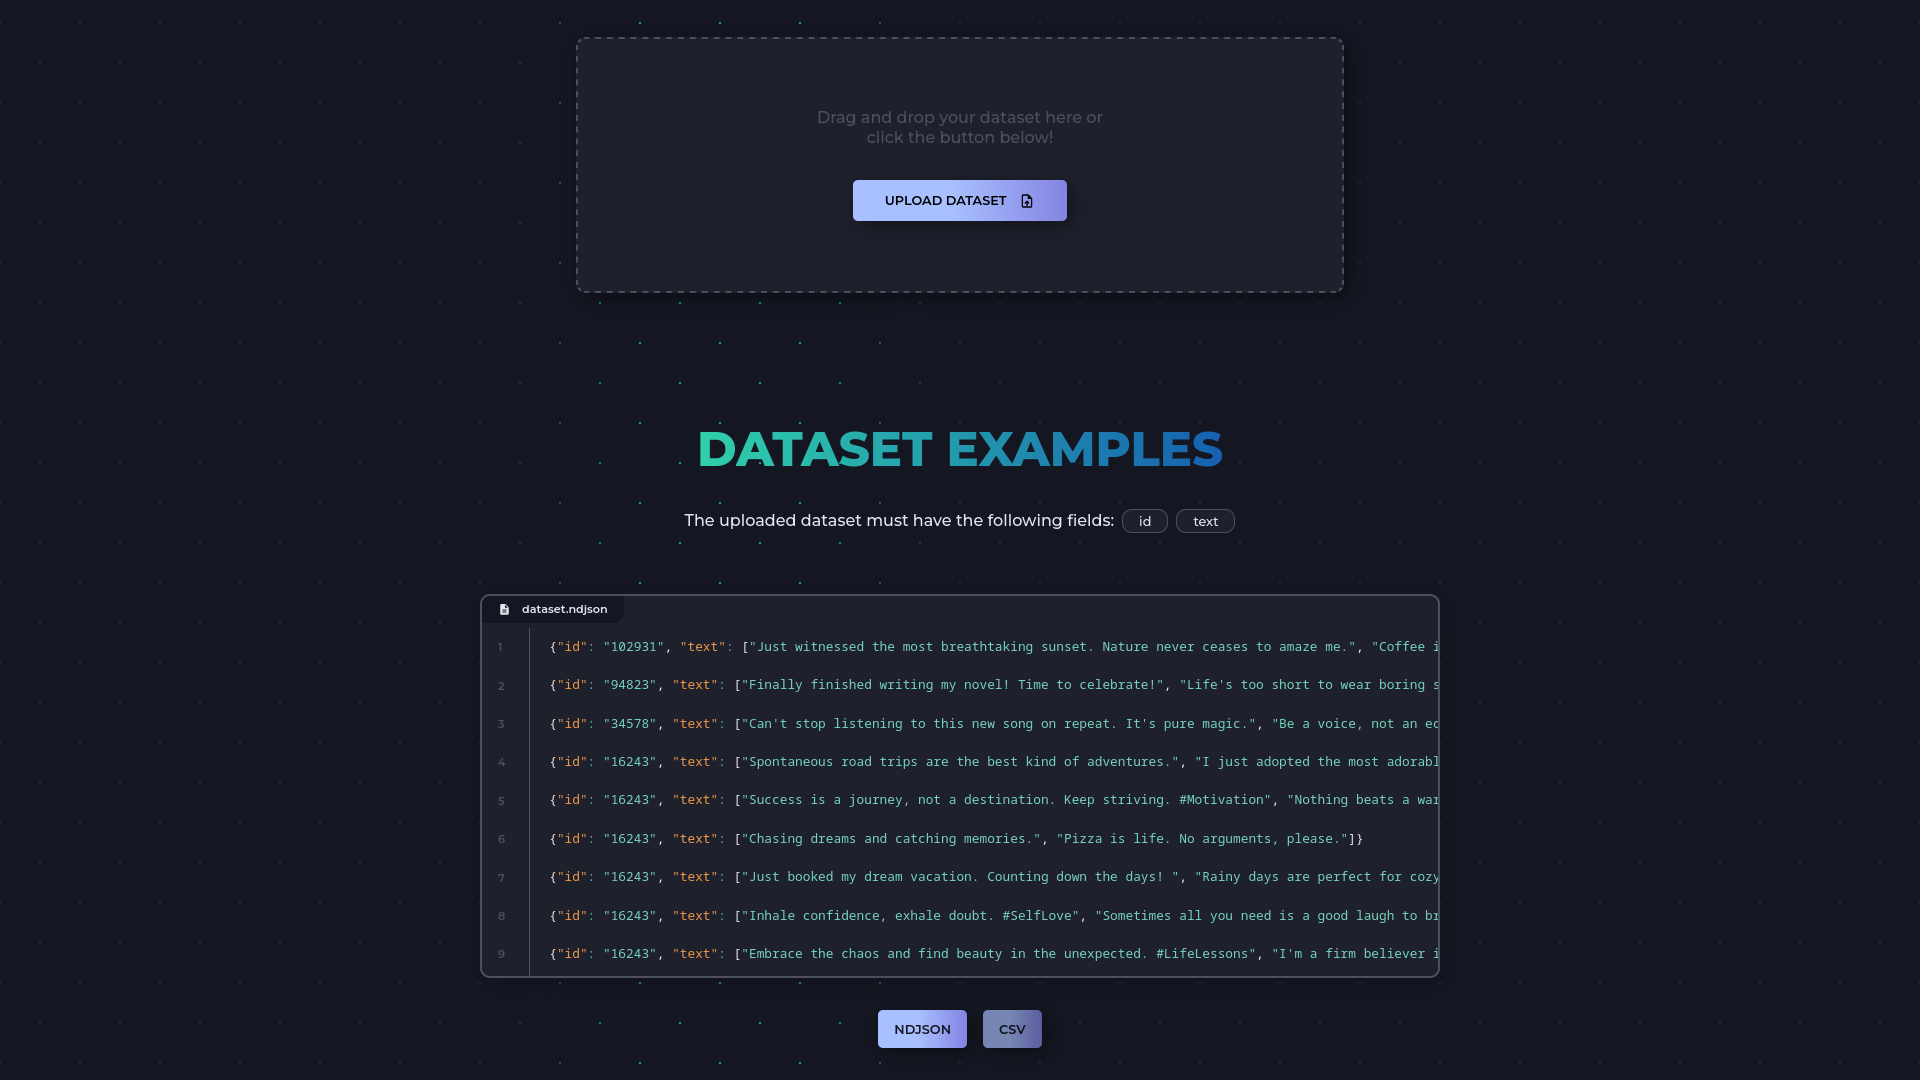
\includegraphics[width=\textwidth]{imagenes/examples.png}
			\label{fig:casouso_examples_escritorio}
	\end{subfigure}
	\hfill
	\begin{subfigure}[c]{0.21\textwidth}
			\centering
			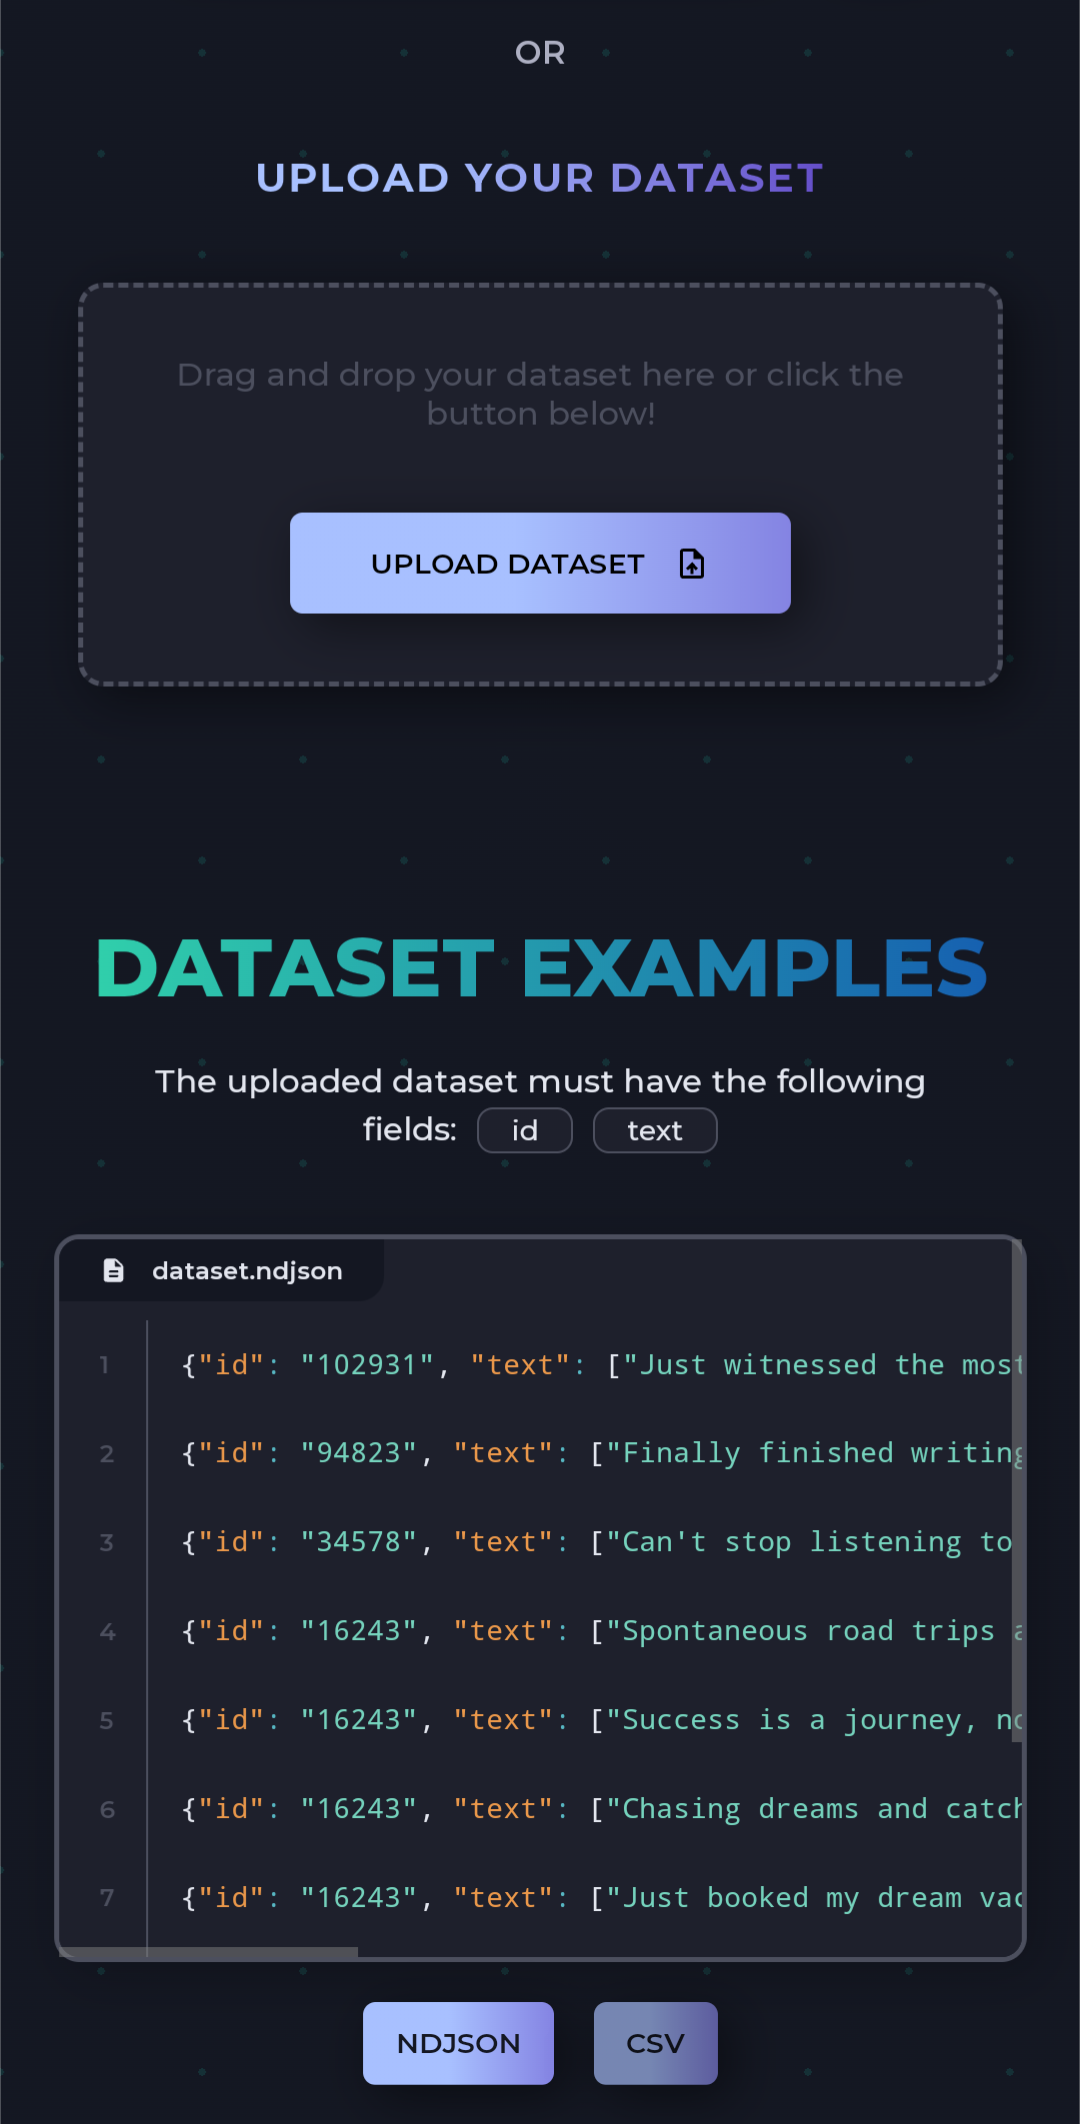
\includegraphics[width=\textwidth]{imagenes/examples_movil.png}
			\label{fig:casouso_examples_movil}
	\end{subfigure}
	\vspace{-1\baselineskip}
	\caption{Página de ejemplos de \textit{datasets}}
	\label{fig:casouso_examples}
\end{figure}

\section{Selección del algoritmo}
\label{sec:casouso_algoritmo}

En este punto, una vez subido el \textit{dataset} deseado, el usuario debe seleccionar el algoritmo de perfilado que más se ajuste
a sus necesidades. En este decisión, es fundamental tener en cuenta el lenguaje en el que se encuentra el \textit{dataset},
las características que se buscan perfilar, el rendimiento del algoritmo o incluso el \textit{dataset} con el que ha sido entrenado.
Así, por un lado se muestran unas tarjetas con la información básica de cada algoritmo, como se puede ver
en la Figura \ref{fig:casouso_algorithms} y, por otro lado, se muestran \textit{tooltips} con información más detallada
sobre el funcionamiento del algoritmo, el \textit{dataset} de entrenamiento y el rendimiento del mismo, 
como se distingue en la Figura \ref{fig:casouso_tooltip}.

\bigskip
\begin{figure}[H]
	\centering
	\begin{subfigure}[c]{0.74\textwidth}
			\centering
			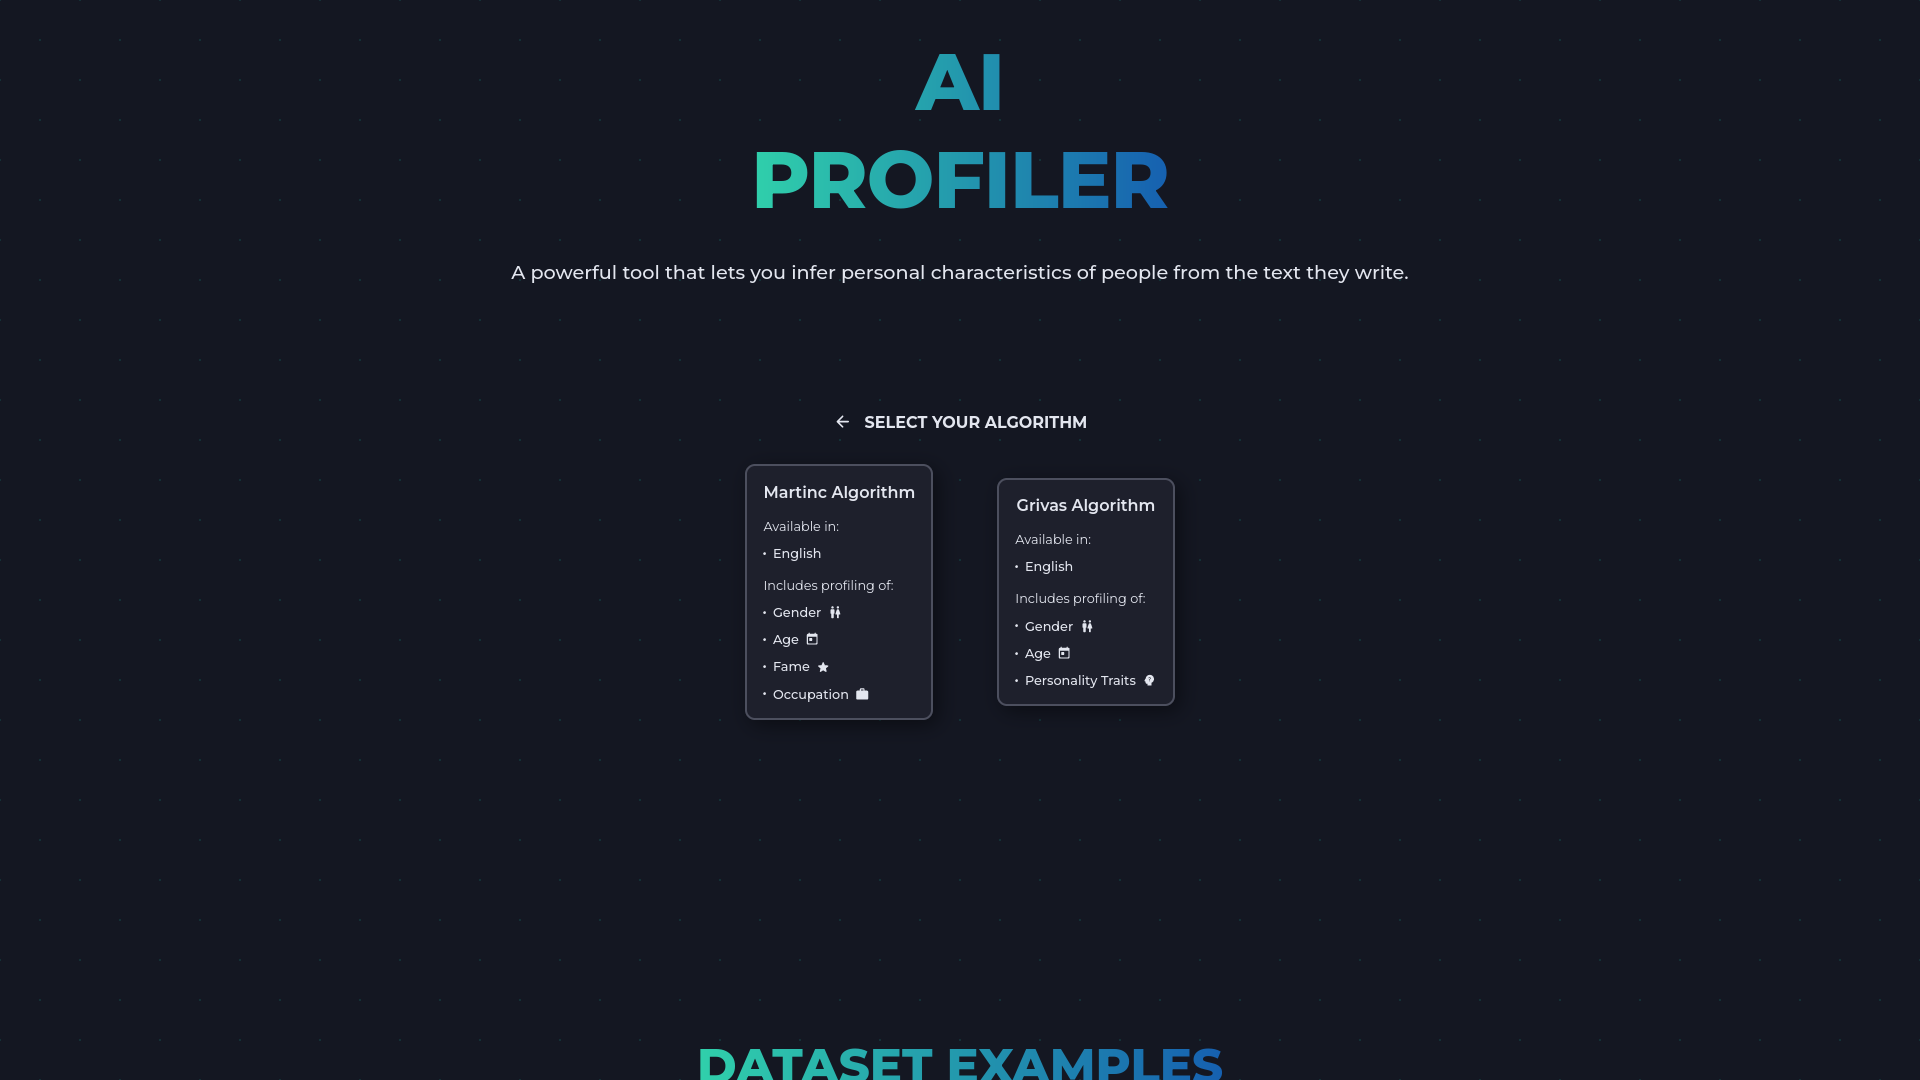
\includegraphics[width=\textwidth]{imagenes/algorithms.png}
			\label{fig:casouso_algorithms_escritorio}
	\end{subfigure}
	\hfill
	\begin{subfigure}[c]{0.21\textwidth}
			\centering
			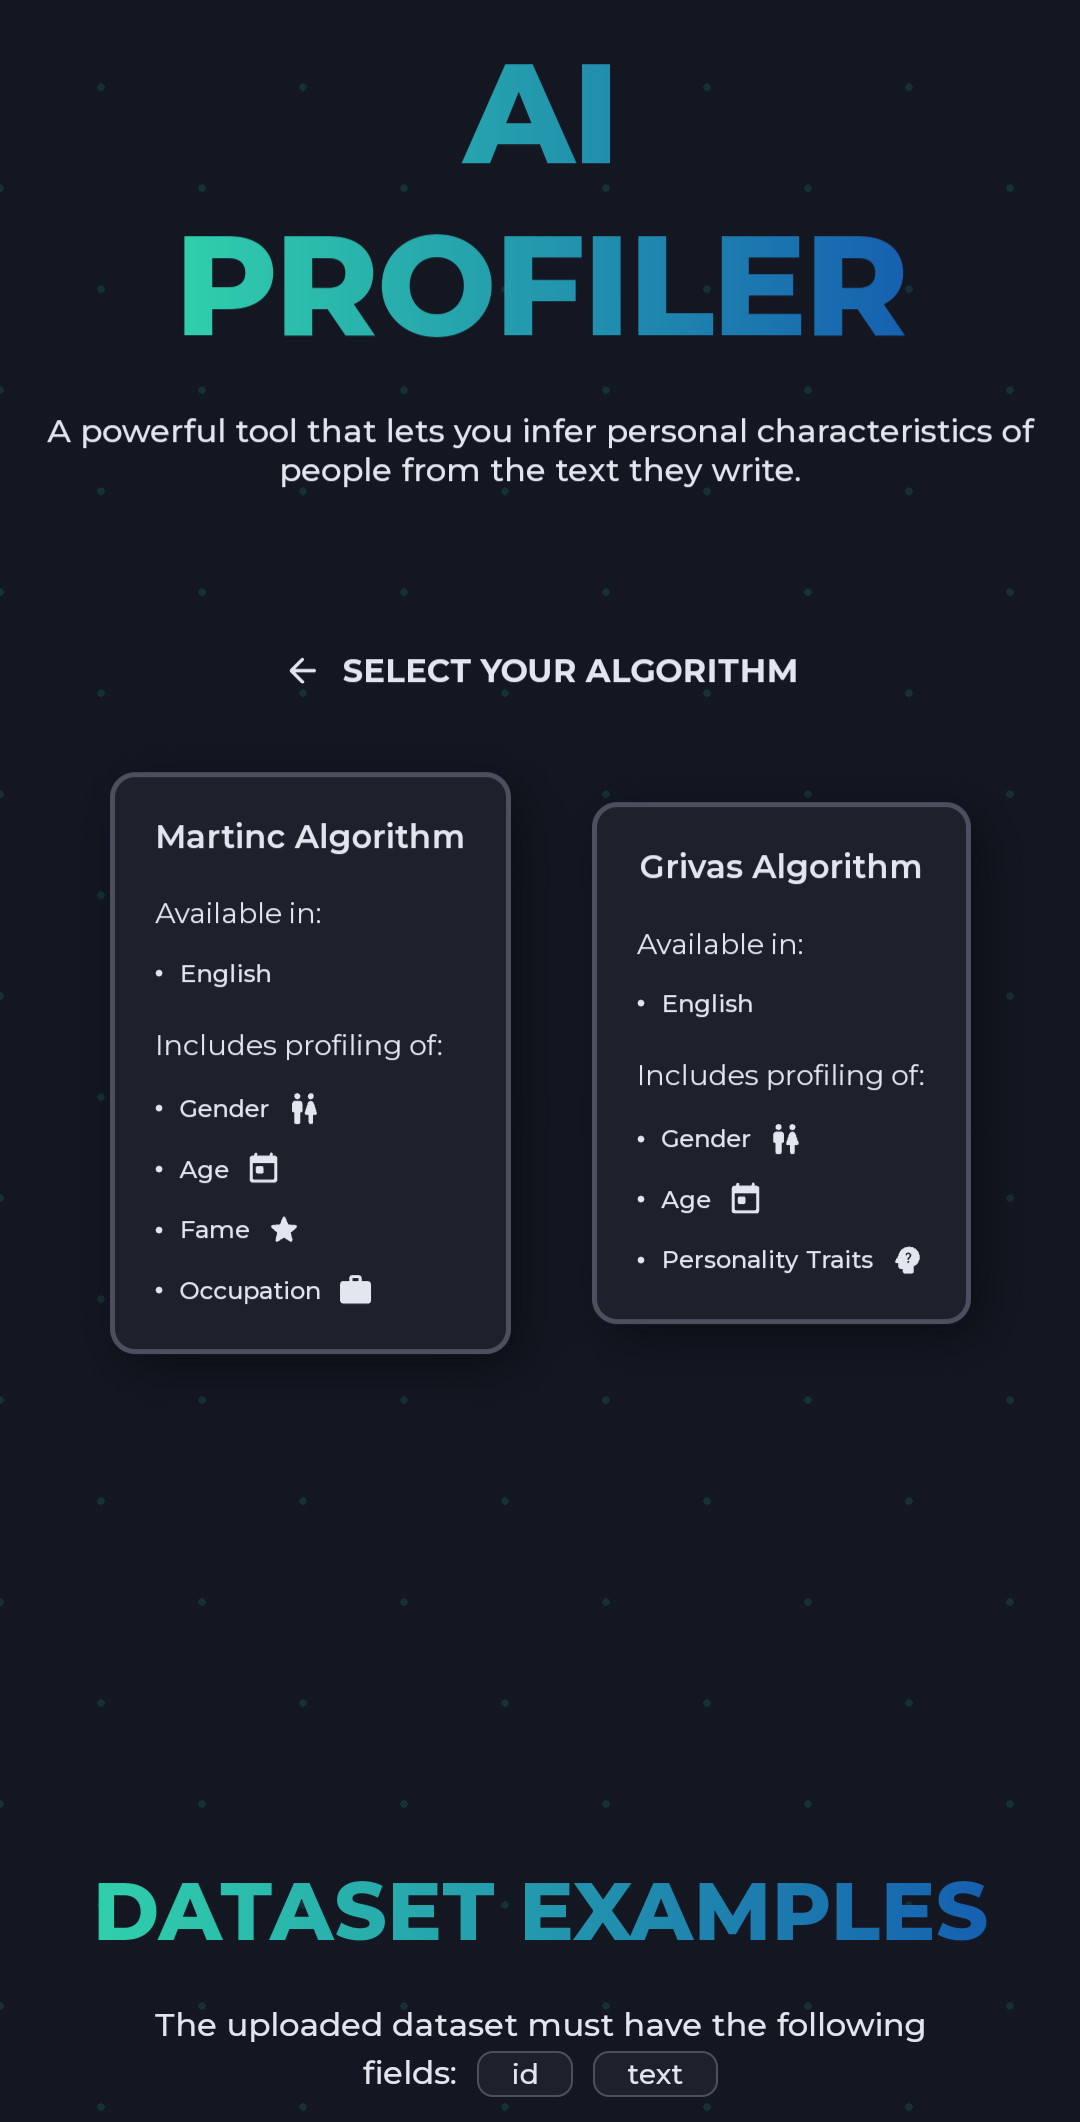
\includegraphics[width=\textwidth]{imagenes/algorithms_movil.png}
			\label{fig:casouso_algorithms_movil}
	\end{subfigure}
	\vspace{-1\baselineskip}
	\caption{Página de selección algoritmos}
	\label{fig:casouso_algorithms}
\end{figure}

\bigskip
\begin{figure}[H]
	\centering
	\begin{subfigure}[c]{0.51\textwidth}
			\centering
			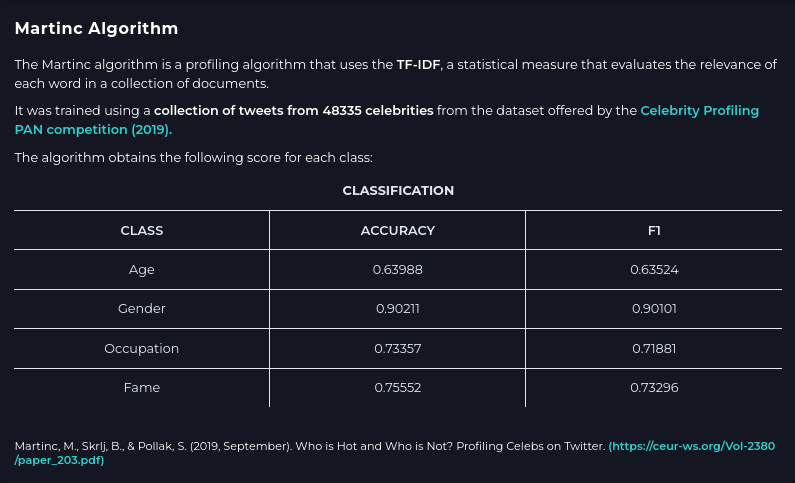
\includegraphics[width=\textwidth]{imagenes/tooltip-martinc.png}
			\label{fig:casouso_tooltip_martinc}
	\end{subfigure}
	\hfill
	\begin{subfigure}[c]{0.46\textwidth}
			\centering
			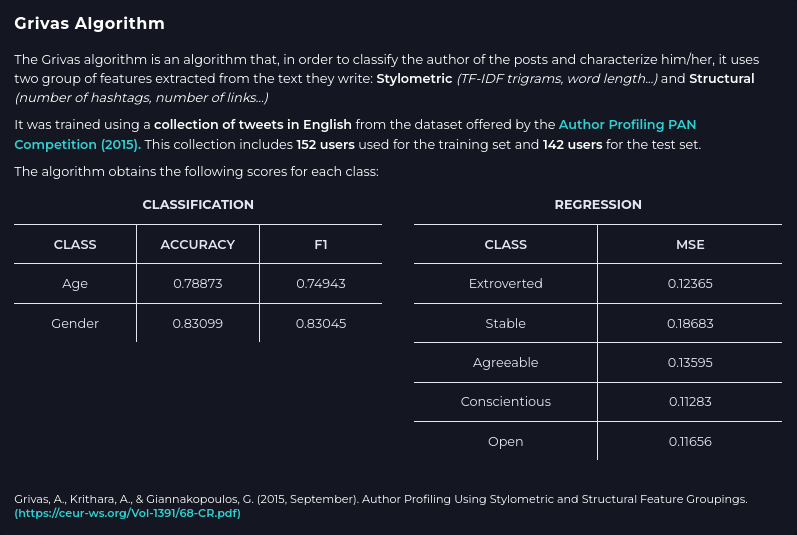
\includegraphics[width=\textwidth]{imagenes/tooltip-grivas.png}
			\label{fig:casouso_tooltip_grivas}
	\end{subfigure}
	\vspace{-1\baselineskip}
	\caption{Tooltip de información sobre los algoritmos}
	\label{fig:casouso_tooltip}
\end{figure}

\section{Proceso de perfilado}
\label{sec:casouso_perfilado}

Después de seleccionar el algoritmo, se muestra una página a modo de resumen, en la que se puede observar el \textit{dataset} subido
junto al algoritmo seleccionado. Para comenzar el proceso de perfilado, el usuario debe pulsar el botón
\textit{Start profiling} y, para proporcionar \textit{feedback} sobre la ejecución del proceso y mejorar la experiencia de usuario,
se muestra una barra de progreso infinita. Esta página puede verse en la Figura \ref{fig:casouso_overview}.

\bigskip
\begin{figure}[H]
	\centering
	\begin{subfigure}[c]{0.74\textwidth}
			\centering
			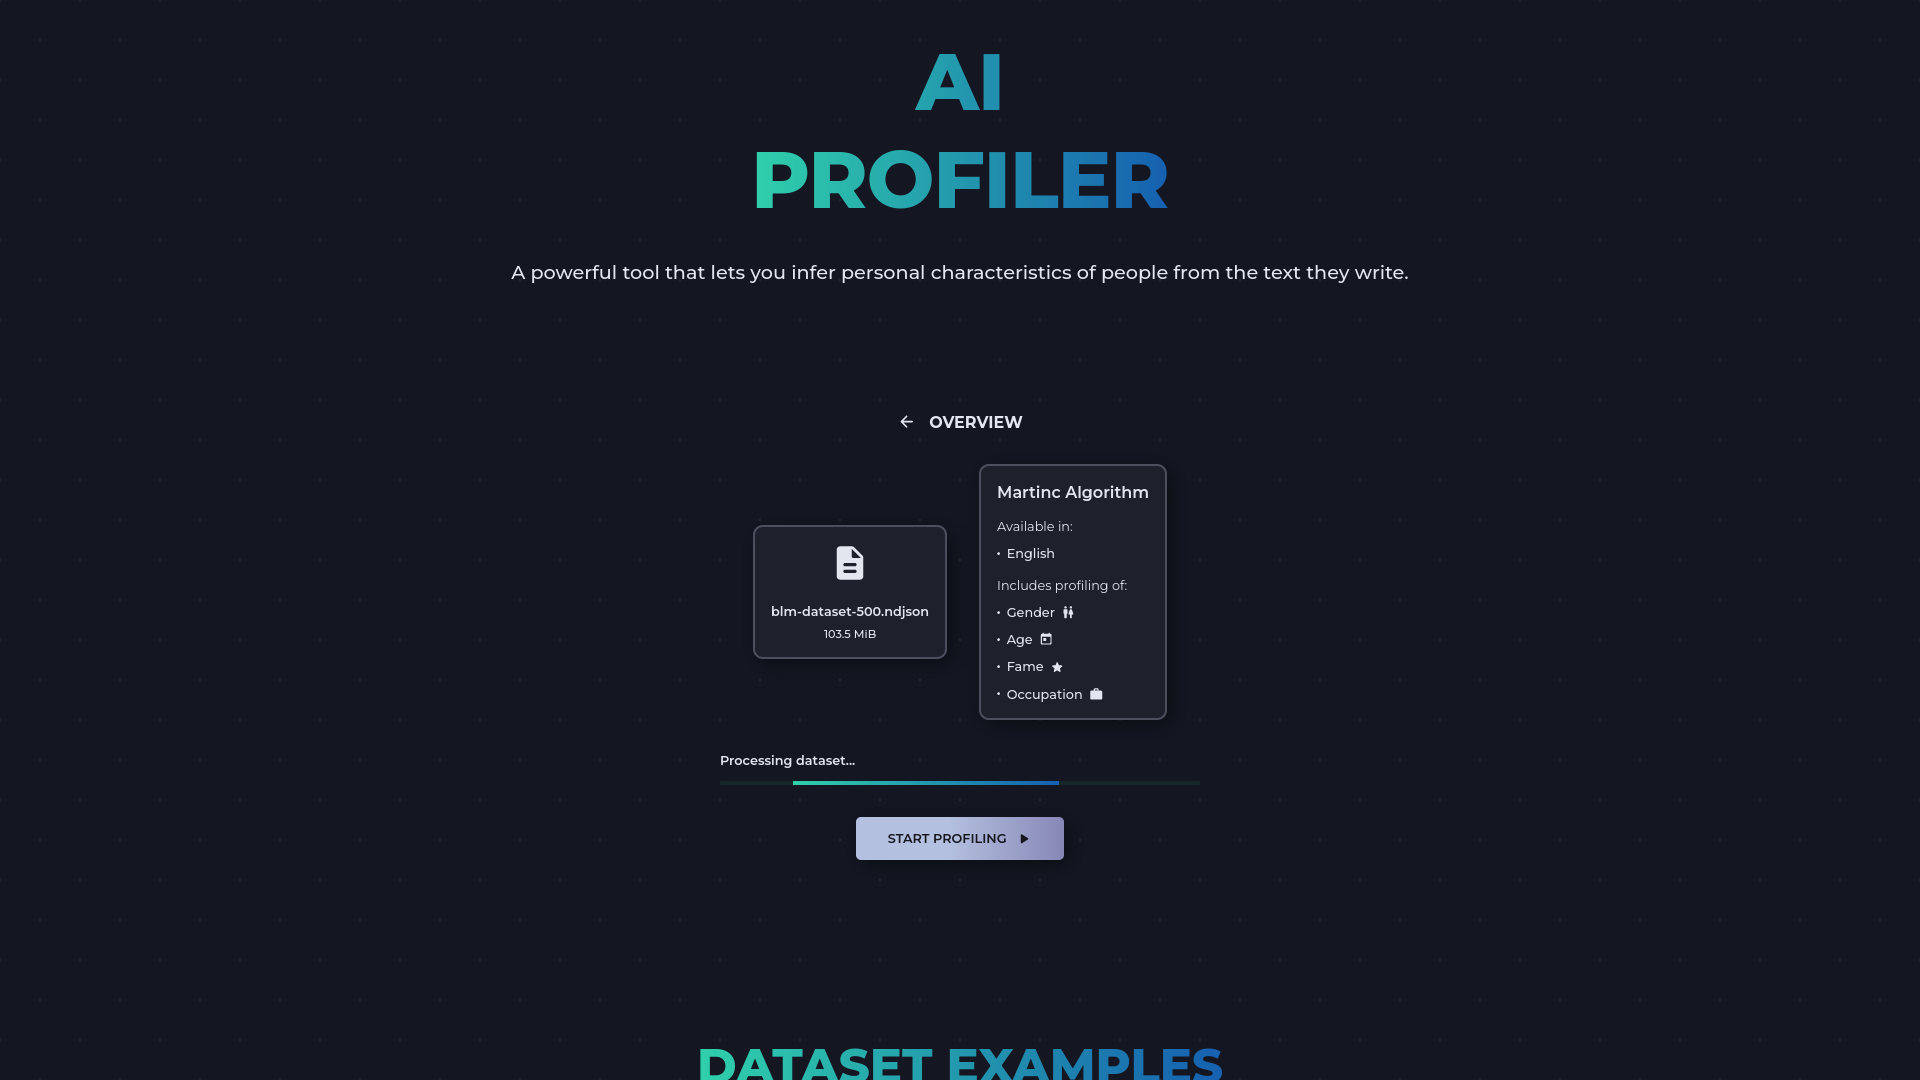
\includegraphics[width=\textwidth]{imagenes/overview.png}
			\label{fig:casouso_overview_escritorio}
	\end{subfigure}
	\hfill
	\begin{subfigure}[c]{0.21\textwidth}
			\centering
			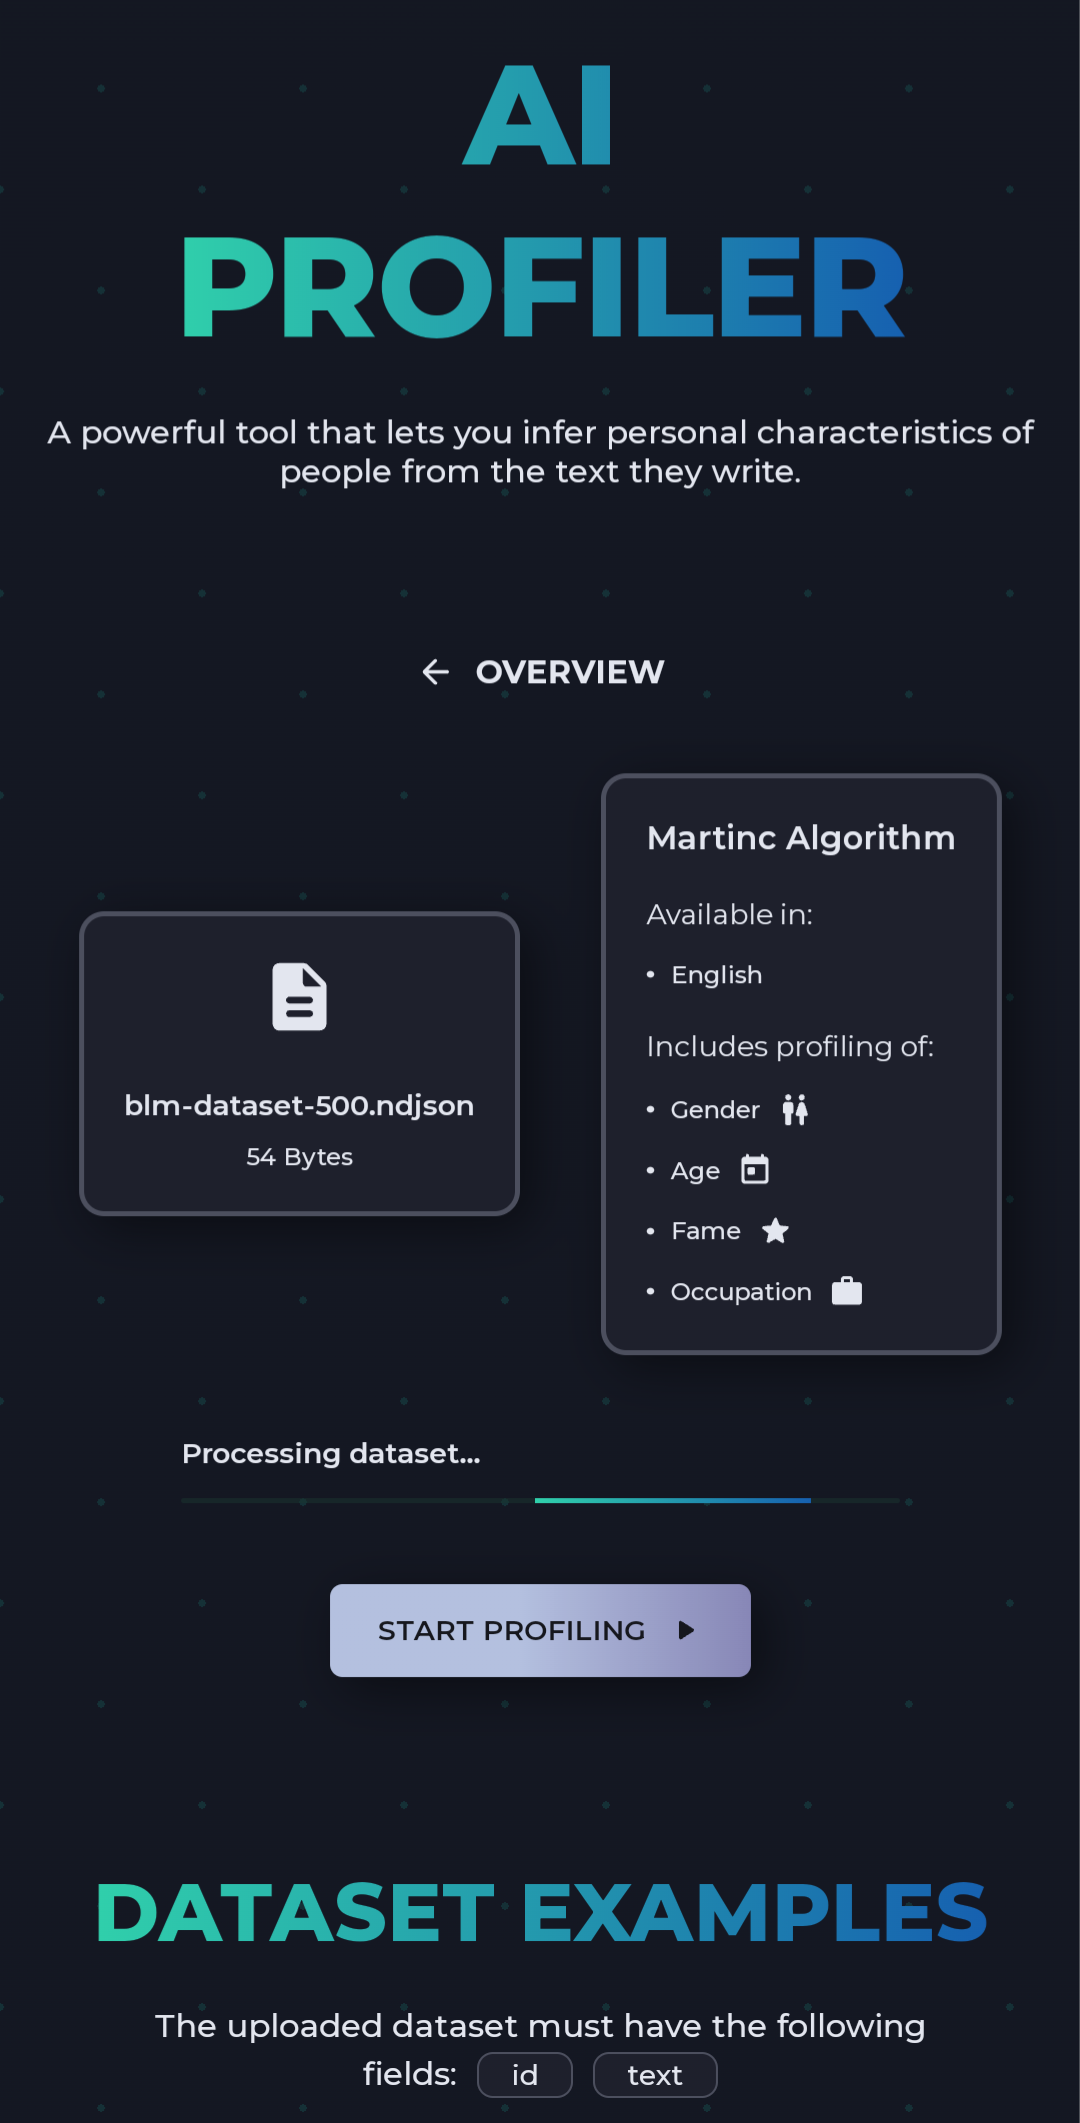
\includegraphics[width=\textwidth]{imagenes/overview_movil.png}
			\label{fig:casouso_overview_movil}
	\end{subfigure}
	\vspace{-1\baselineskip}
	\caption{Página de resumen del perfilado}
	\label{fig:casouso_overview}
\end{figure}

\section{Visualización de resultados}
\label{sec:casouso_dashboard}

Tras finalizar el proceso de perfilado, se muestra una página con los resultados obtenidos en formato \textit{dashboard}, al igual
que se especificaba en los prototipos de la Sección \ref{sec:diseño_prototipado}. De esta forma, el \textit{dashboard} fue
implementado teniendo como objetivo principal que toda la información estuviera disponible en una única página en la que se
mostraran únicamente datos relevantes para el usuario, sin necesidad de hacer \textit{scroll} para verla. Asimismo, en función del algoritmo
empleado, se muestran unos gráficos u otros, como se puede ver en las Figuras \ref{fig:casouso_dashboard_martinc} y
\ref{fig:casouso_dashboard_grivas}.

\bigskip
\begin{figure}[H]
	\centering
	\begin{subfigure}[c]{0.74\textwidth}
			\centering
			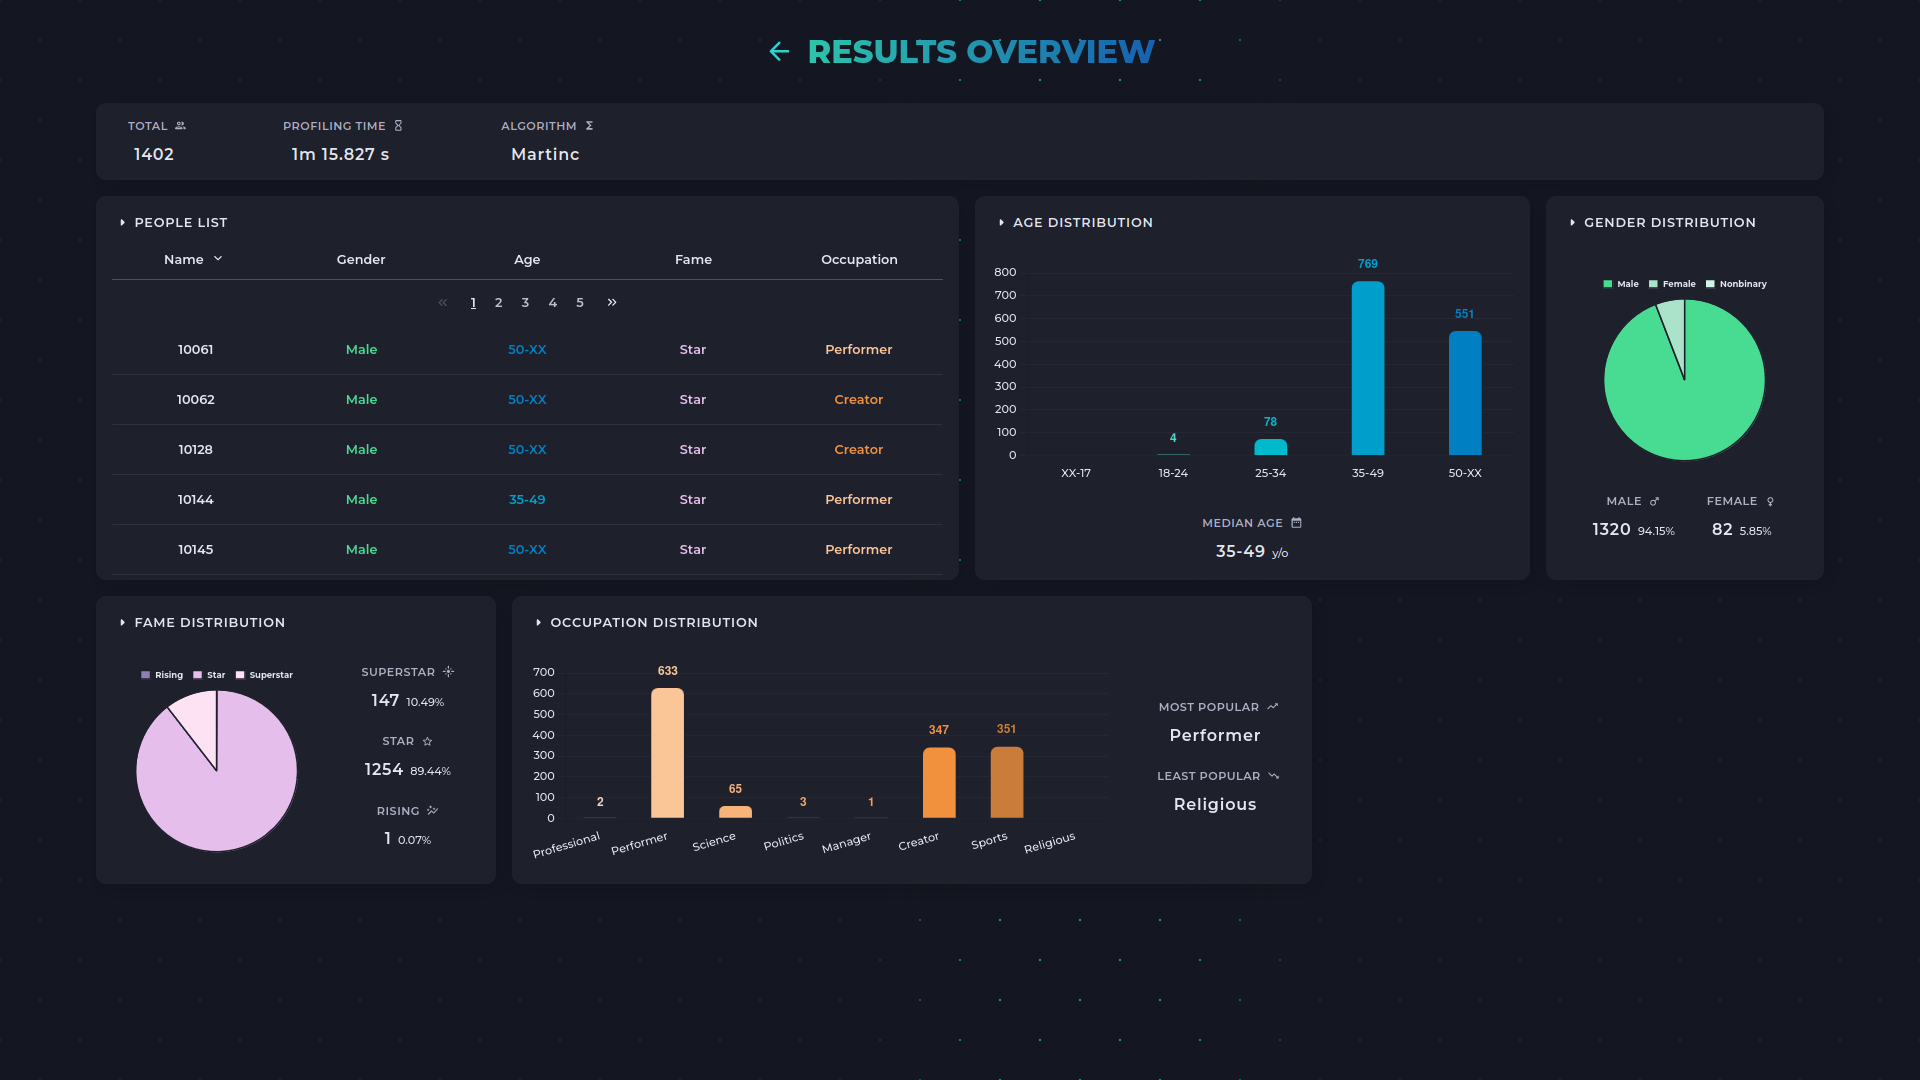
\includegraphics[width=\textwidth]{imagenes/dashboard-martinc-500.png}
			\label{fig:casouso_dashboard_martinc_escritorio}
	\end{subfigure}
	\hfill
	\begin{subfigure}[c]{0.21\textwidth}
			\centering
			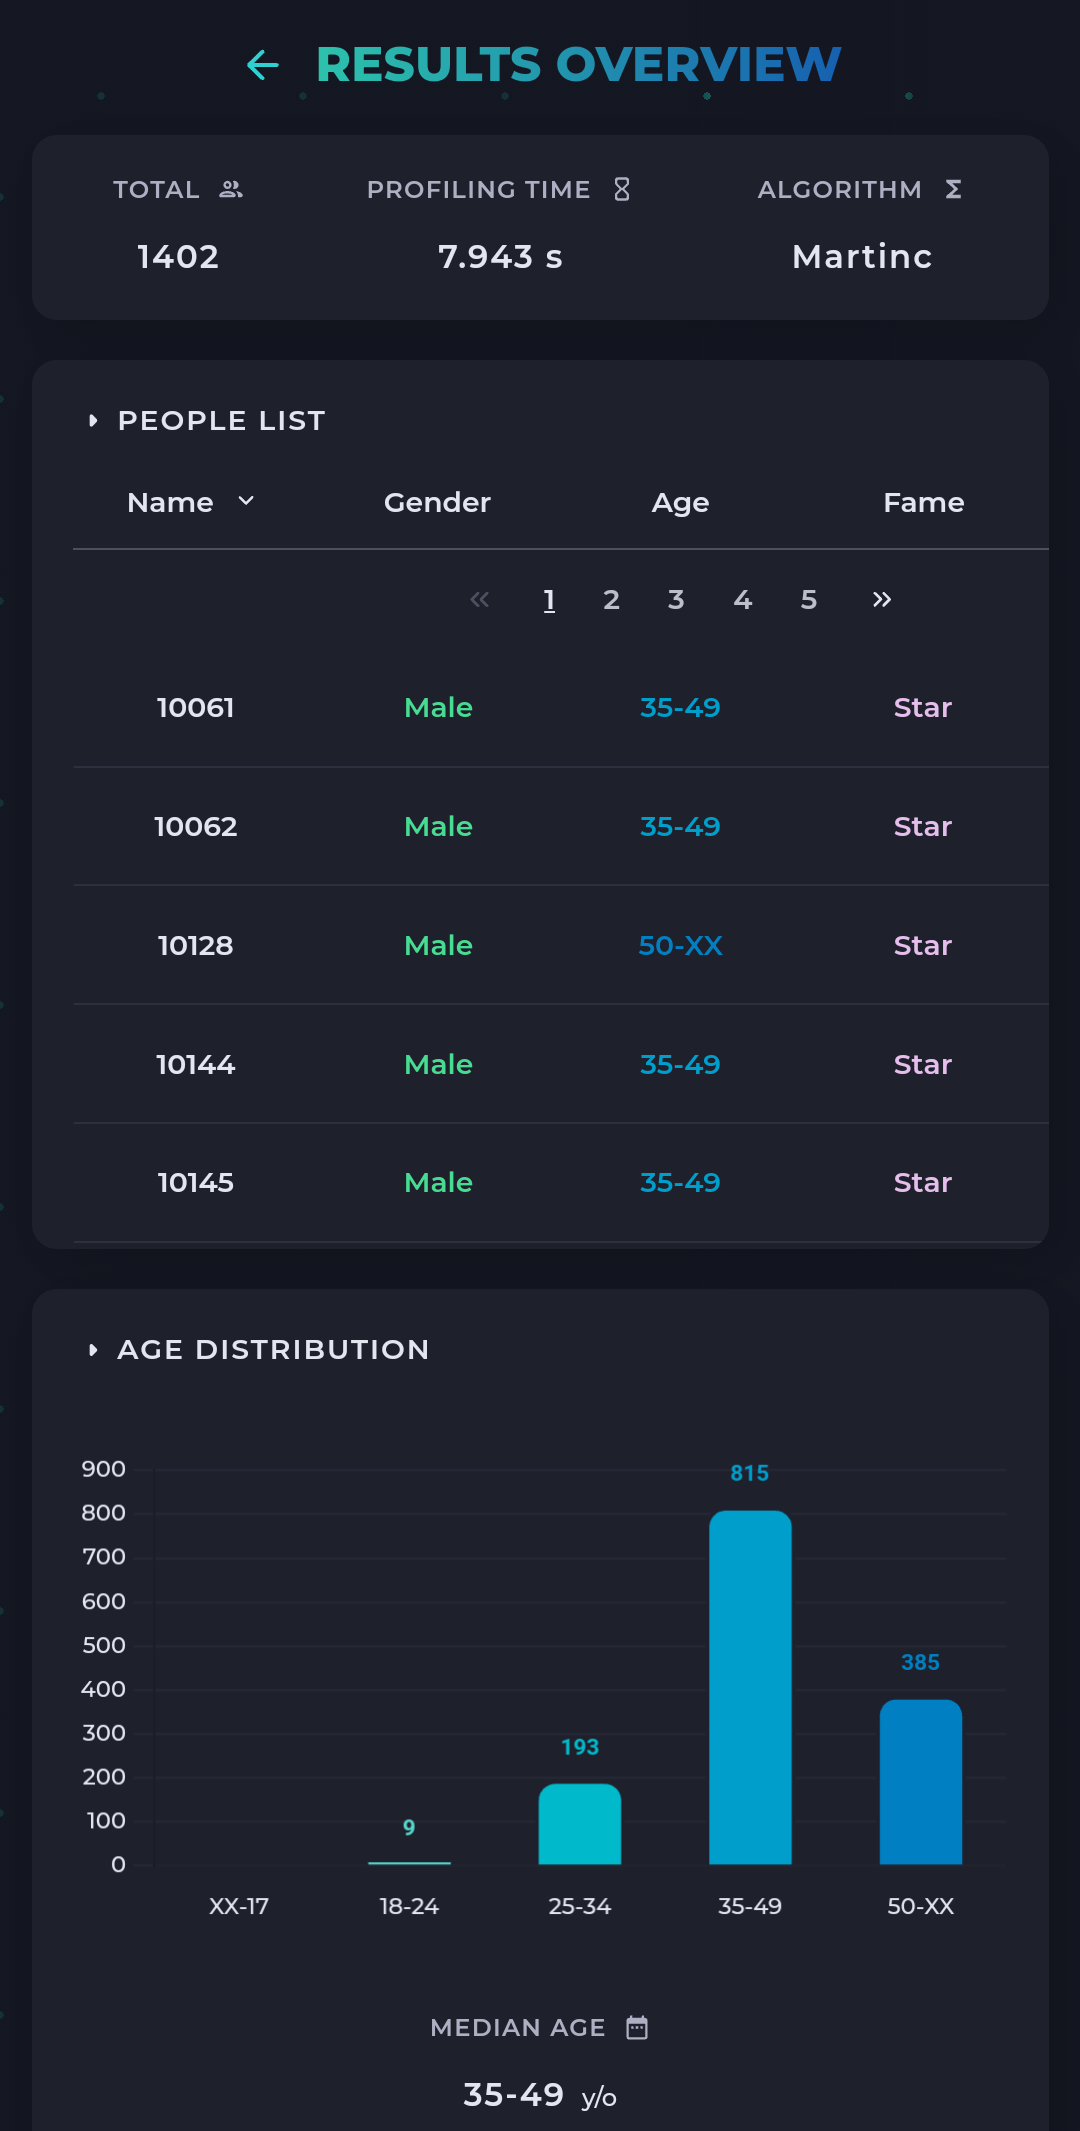
\includegraphics[width=\textwidth]{imagenes/dashboard-martinc-500_movil.png}
			\label{fig:casouso_dashboard_martinc_movil}
	\end{subfigure}
	\vspace{-1\baselineskip}
	\caption{Dashboard con los resultados obtenidos por el algoritmo de Martinc \cite{martinc2019hot}}
	\label{fig:casouso_dashboard_martinc}
\end{figure}

\begin{figure}[H]
	\centering
	\begin{subfigure}[c]{0.74\textwidth}
			\centering
			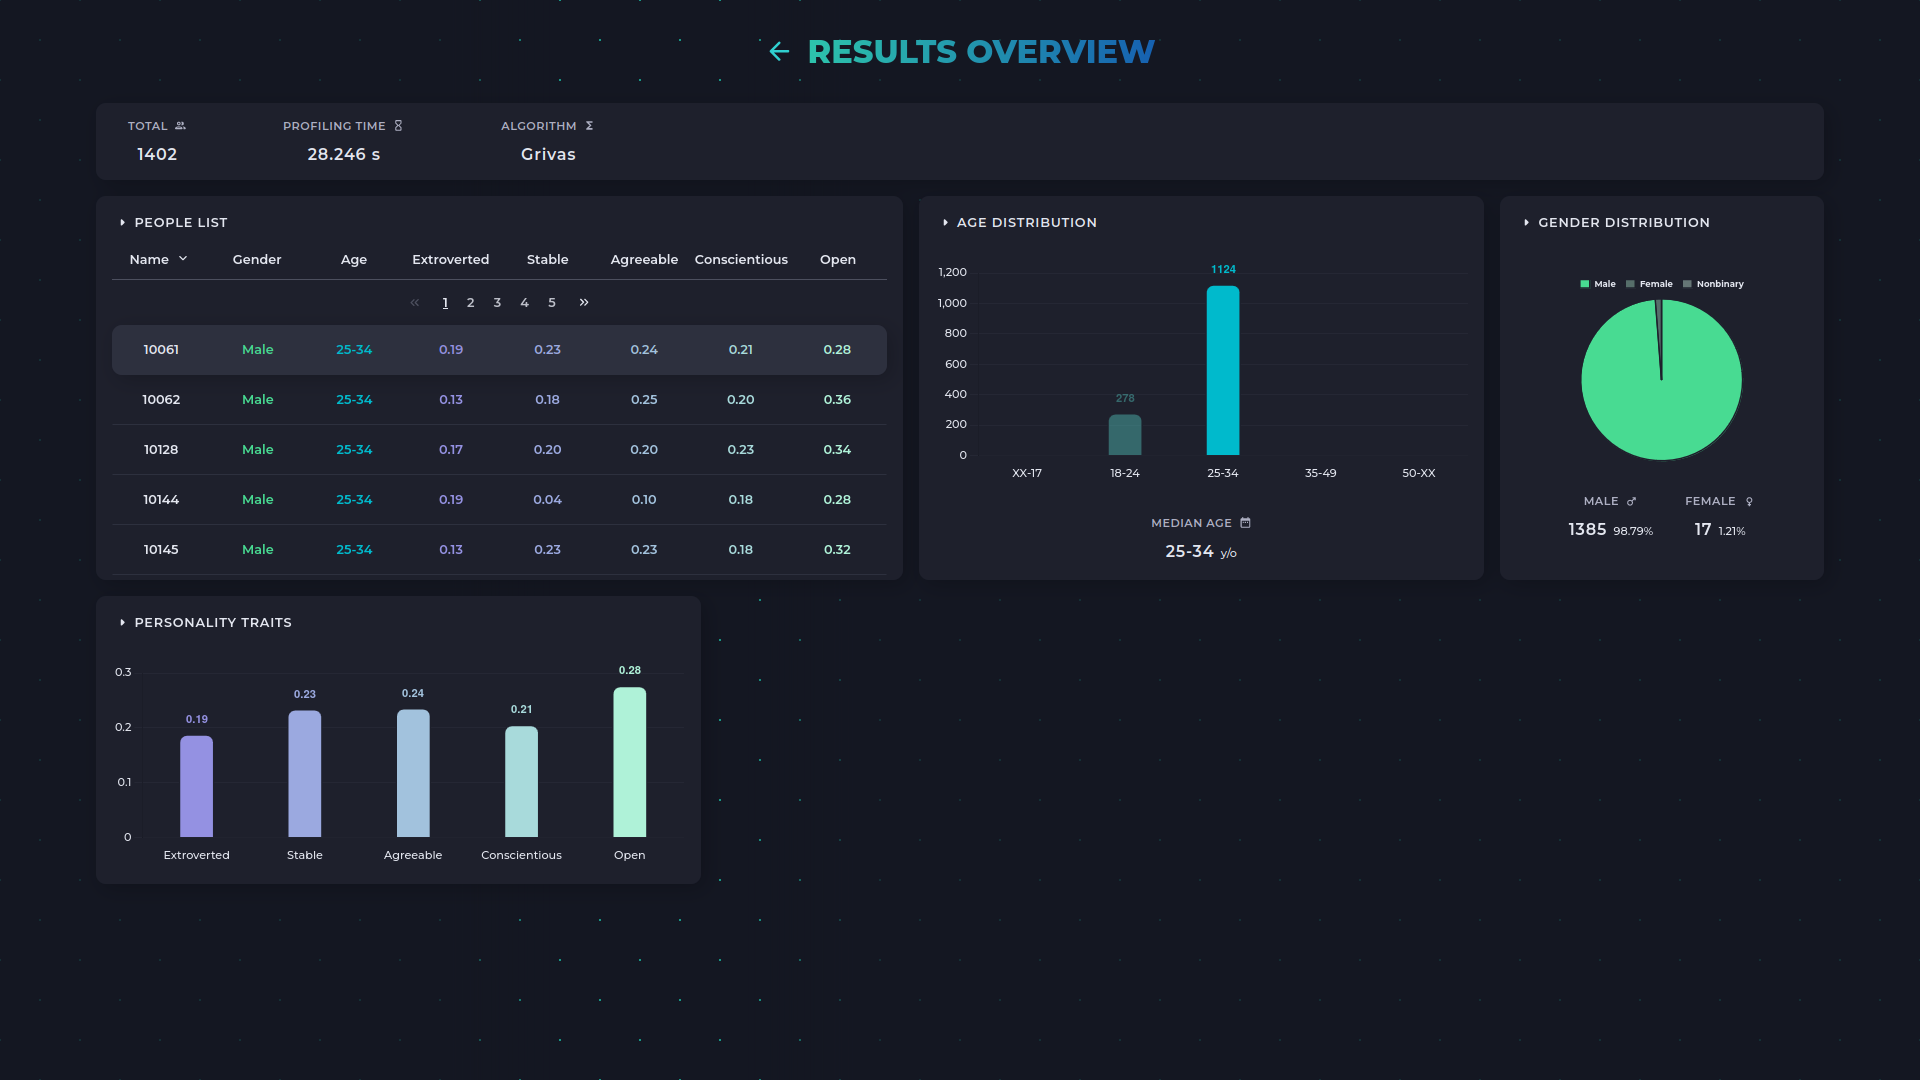
\includegraphics[width=\textwidth]{imagenes/dashboard-grivas-500.png}
			\label{fig:casouso_dashboard_grivas_escritorio}
	\end{subfigure}
	\hfill
	\begin{subfigure}[c]{0.21\textwidth}
		\centering
		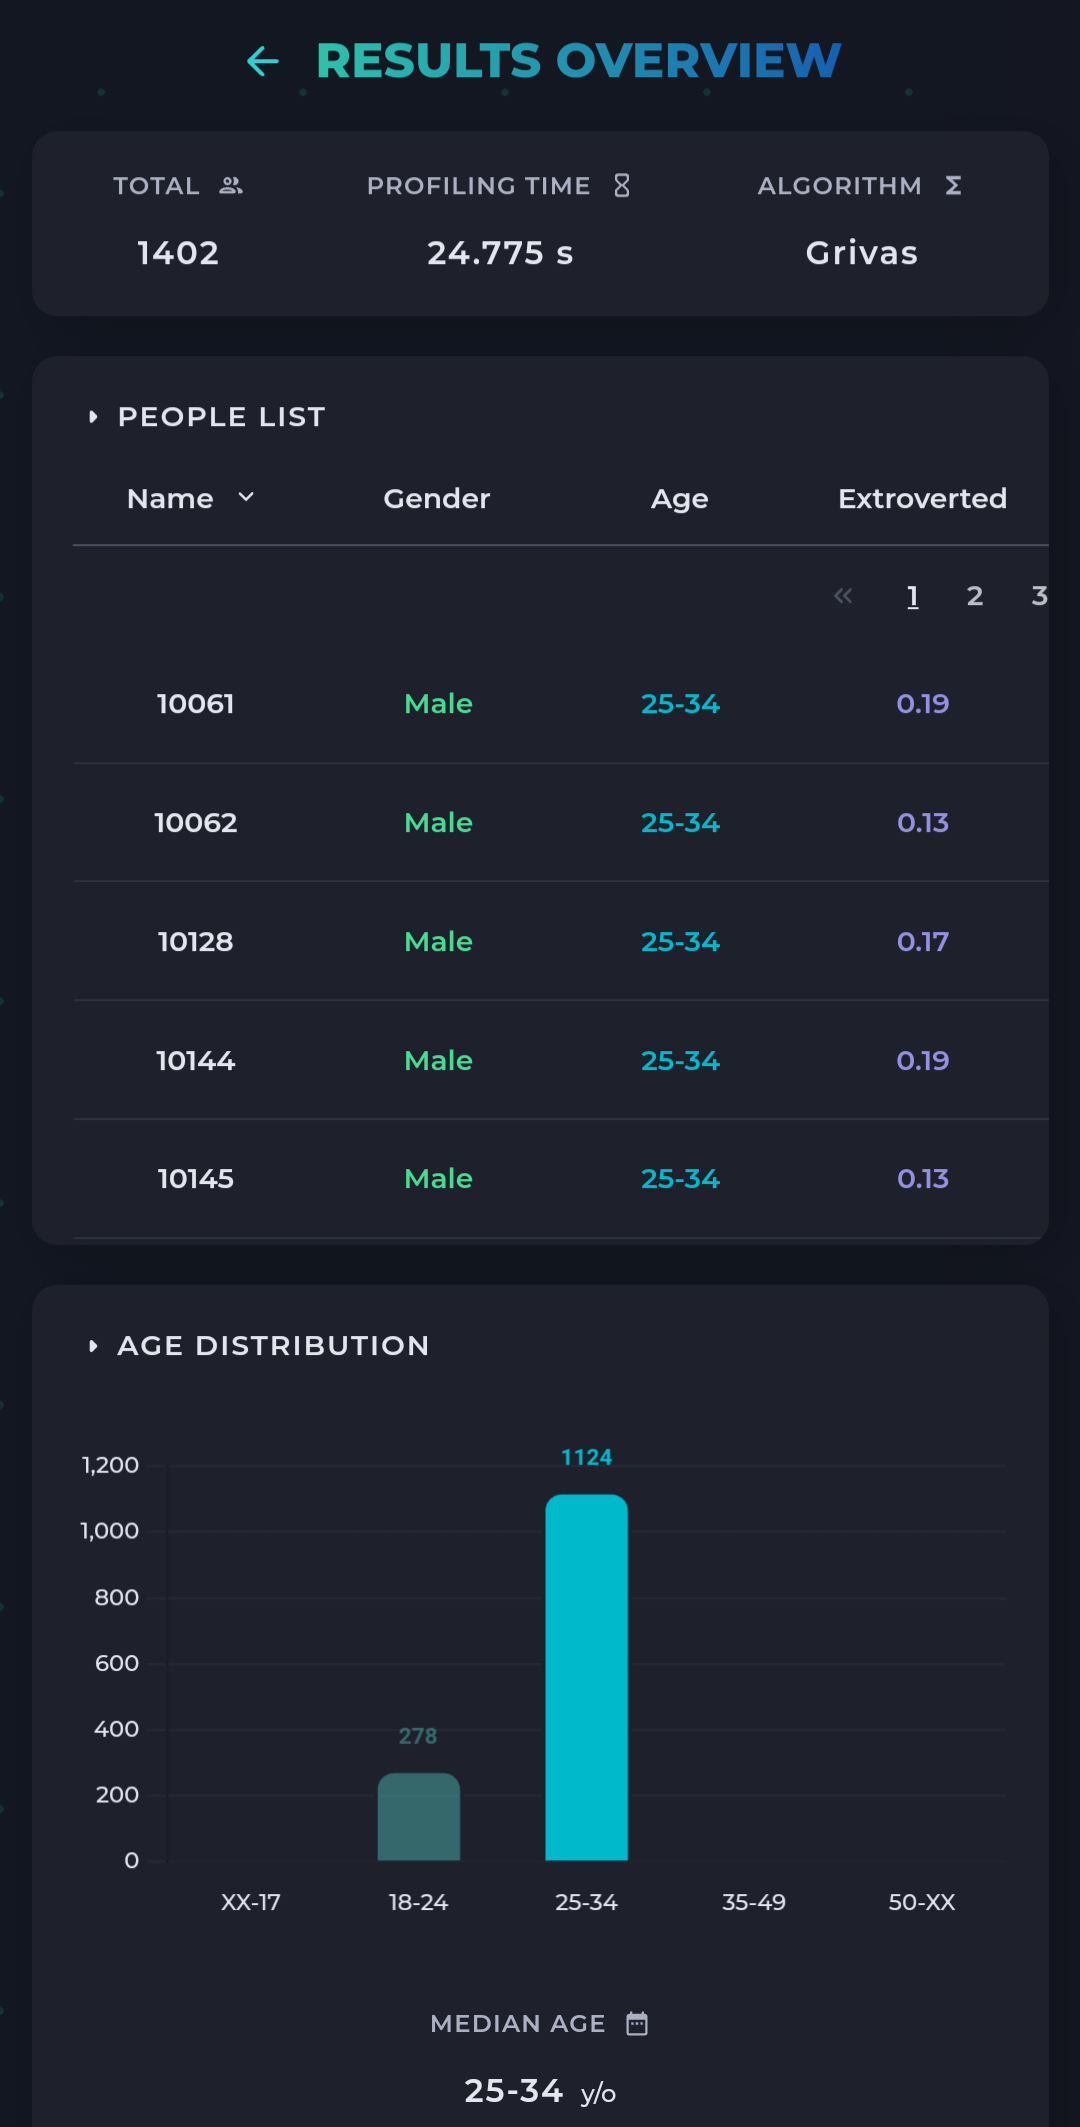
\includegraphics[width=\textwidth]{imagenes/dashboard-grivas-500_movil.png}
		\label{fig:casouso_dashboard_grivas_movil}
	\end{subfigure}
	\vspace{-1\baselineskip}
	\caption{Dashboard con los resultados obtenidos por el algoritmo de Grivas \cite{grivas2015author}}
	\label{fig:casouso_dashboard_grivas}
\end{figure}

\section{Análisis de resultados}
\label{sec:casouso_analisis}

Para llevar a cabo el análisis de los resultados obtenidos, se abordará el estudio de cada característica por separado y se
comprarán las predicciones realizadas por ambos algoritmos. A mayores, y a modo de experimentación para comprobar las diferencias subyacentes en el perfilado, 
se hará uso de tres \textit{datasets} con diferente número de posts por usuario, como se comentó en la Sección \ref{sec:casouso_dataset}.

\bigskip
En cuanto a la distribución de género, como se aprecia en la Tabla \ref{tab:comparativa_genero}, vemos como ambos algoritmos otorgan una gran mayoría al género masculino en cualquiera de
los tres \textit{datasets}. En el caso del algoritmo de Grivas \cite{grivas2015author}, observamos como a medida que aumenta el número de posts por usuario
el número de usuarios clasificados como femeninos disminuye excesivamente. Esto quizá es debido al limitado \textit{dataset} utilizado
para entrenar dicho algoritmo, de apenas 150 personas, por lo que es posible que no sea lo suficientemente representativo. En lo que respecta
al algoritmo de Martinc \cite{martinc2019hot}, vemos como al aumentar el número de posts por usuario, el número de usuarios clasificados como masculinos
se estabiliza alrededor de 1320 (94\%), mientras que el número de usuarios clasificados como femeninos se queda en 82 (6\%). Esta diferencia
tan amplia, sin embargo, no tiene una clara relación con la realidad ya que según Statista, la distribución de género en Reddit es
de un 64\% para hombres y un 36\% para mujeres \cite{statistagenero}, aunque esta proporción puede variar en función
de la comunidad o del tema que se trate.

\begin{table}[H]
	\centering
	\resizebox{0.8\textwidth}{!}{
		\rowcolors{2}{white}{udcgray!25}
		\begin{tabular}{|c|c|c|c|c|}
			\hhline{~|----|}
			\multicolumn{1}{c|}{\cellcolor{white}} & \multicolumn{2}{c|}{\cellcolor{udcpink!25}\textbf{Martinc}} & \multicolumn{2}{c|}{\cellcolor{udcpink!25}\textbf{Grivas}} \\ \hline
			\multicolumn{1}{|c|}{\textbf{Posts/usuario}} & \multicolumn{1}{c|}{\textbf{Male}} & \multicolumn{1}{c|}{\textbf{Female}} &
			\multicolumn{1}{c|}{\textbf{Male}} & \multicolumn{1}{c|}{\textbf{Female}} \\ \hline
			50 & 1294 & 108 & 1385 & 17 \\ \hline
			500 & 1320 & 82 & 1400 & 2 \\ \hline
			1000 & 1318 & 84 & 1400 & 2 \\ \hline
		\end{tabular}
	}
	\caption{Distribución de género obtenida en ambos algoritmos}
	\label{tab:comparativa_genero}
\end{table}

\bigskip
En el caso de la distribución de edad, ambos algoritmos reflejan amplias diferencias en los resultados obtenidos, como se puede
ver en las Tablas \ref{tab:comparativa_edad_martinc} y \ref{tab:comparativa_edad_grivas}. En el caso del algoritmo de Martinc \cite{martinc2019hot}, observamos
como, a medida que aumenta el número de posts por usuario, el número de usuarios pertenecientes a la franja de edad 50-XX aumenta
considerablemente, mientras que el número de usuarios pertenecientes a la franja de edad 35-49 disminuye. En este caso, debido al gran
número de usuarios utilizados para el entrenamiento, cerca de 20.000, junto al gran rendimiento que demostraba en cuanto a precisión,
es posible que, al contar con más posts y, por ende, con más información por usuario, el algoritmo sea capaz de realizar una clasificación
más precisa. En cuanto a los datos obtenidos en la encuesta llevada a cabo por Statista a la población estadounidense adulta en 2021,
la distribución de edad en Reddit es de un 36\% para
los usuarios de entre 18 y 29 años, un 22\% para los usuarios de entre 30 y 49 años y un 13\% para los usuarios de entre 50 y más \cite{statistaedad}.
Esto puede indicar que, debido a que el número de usuarios perfilados por el algoritmo entre 18 y 34 años es de tan solo un 5\%, son los usuarios
con más edad los que participan en debates políticos como el caso del BLM.
Pasando al algoritmo de Grivas \cite{grivas2015author} y de la misma forma que sucedía con la distribución de género, los resultados obtenidos
parecen estar la mayor parte concentrados en una única clase, en este caso la de 25-34 años, por lo que esto puede deberse, de nuevo, al limitado
número de usuarios utilizados para entrenar el algoritmo.

\begin{table}[H]
	\centering
	\resizebox{0.8\textwidth}{!}{
		\rowcolors{2}{white}{udcgray!25}
		\begin{tabular}{|c|c|c|c|c|c|}
			\hhline{~|-----|}
			\multicolumn{1}{c|}{\cellcolor{white}} & \multicolumn{5}{c|}{\cellcolor{udcpink!25}\textbf{Martinc}} \\ \hline
			\textbf{Posts/usuario} & \textbf{XX-17} & \textbf{18-24} & \textbf{25-34} & \textbf{35-49} & \textbf{50-XX} \\ \hline
			50 & 0 & 9 & 193 & 815 & 385 \\ \hline
			500 & 0 & 4 & 78 & 769 & 551 \\ \hline
			1000 & 0 & 4 & 63 & 665 & 670 \\ \hline
		\end{tabular}
	}
	\caption{Distribución de edad obtenida por Martinc \cite{martinc2019hot}}
	\label{tab:comparativa_edad_martinc}
\end{table}

\begin{table}[H]
	\centering
	\resizebox{0.8\textwidth}{!}{
		\rowcolors{2}{white}{udcgray!25}
		\begin{tabular}{|c|c|c|c|c|c|}
			\hhline{~|-----|}
			\multicolumn{1}{c|}{\cellcolor{white}} & \multicolumn{5}{c|}{\cellcolor{udcpink!25}\textbf{Grivas}} \\ \hline
			\textbf{Posts/usuario} & \textbf{XX-17} & \textbf{18-24} & \textbf{25-34} & \textbf{35-49} & \textbf{50-XX} \\ \hline
			50 & 0 & 278 & 1124 & 0 & 0 \\ \hline
			500 & 0 & 170 & 1232 & 0 & 0 \\ \hline
			1000 & 0 & 168 & 1234 & 0 & 0 \\ \hline
		\end{tabular}
	}
	\caption{Distribución de edad obtenida por Grivas \cite{grivas2015author}}
	\label{tab:comparativa_edad_grivas}
\end{table}

\bigskip
Por último, en cuanto a las características perfiladas únicamente por el algoritmo de Martinc \cite{martinc2019hot}, vemos como apenas hay diferencias notables
en función del número de posts por usuario. Como se puede ver en la Tabla \ref{tab:comparativa_ocupacion_martinc}, la mayoría de los usuarios
son clasificados como \textit{Performer}, \textit{Creator} o \textit{Sports}, mientras que el resto de ocupaciones apenas tienen presencia. En cuanto
al nivel de fama o popularidad de los usuarios, reflejado en la Tabla \ref{tab:comparativa_fama_martinc}, vemos como la gran mayoría de los usuarios
son clasificados como \textit{Star} y el número de usuarios clasificados como \textit{Rising} es prácticamente nulo. Ambas caracterísitcas, al estar
específicamente pensadas para el perfilado de celebridades no son, por lo tanto, determinantes para el \textit{dataset} que estamos analizando.

\bigskip
\begin{table}[H]
	\centering
	\resizebox{\textwidth}{!}{
		\rowcolors{2}{white}{udcgray!25}
		\setlength{\tabcolsep}{7pt}
		\begin{tabular}{|c|c|c|c|c|c|c|c|c|}
			\hhline{~|--------|}
			\multicolumn{1}{c|}{\cellcolor{white}} & \multicolumn{8}{c|}{\cellcolor{udcpink!25}\textbf{Martinc}} \\ \hline
			\textbf{Posts/usuario} & \textbf{Professional} & \textbf{Performer} & \textbf{Science} & \textbf{Politics} & \textbf{Manager} & \textbf{Creator} & \textbf{Sports} & \textbf{Religious} \\ \hline
			50 & 3 & 483 & 43 & 9 & 3 & 390 & 471 & 0 \\ \hline
			500 & 2 & 633 & 65 & 3 & 1 & 347 & 351 & 0 \\ \hline
			1000 & 2 & 691 & 73 & 3 & 1 & 321 & 311 & 0 \\ \hline
		\end{tabular}
	}
	\caption{Distribución de ocupación obtenida por Martinc \cite{martinc2019hot}}
	\label{tab:comparativa_ocupacion_martinc}
\end{table}

\bigskip
\begin{table}[H]
	\centering
	\resizebox{0.6\textwidth}{!}{
		\rowcolors{2}{white}{udcgray!25}
		\begin{tabular}{|c|c|c|c|}
			\hhline{~|---|}
			\multicolumn{1}{c|}{\cellcolor{white}} & \multicolumn{3}{c|}{\cellcolor{udcpink!25}\textbf{Martinc}} \\ \hline
			\textbf{Posts/usuario} & \textbf{Rising} & \textbf{Star} & \textbf{Superstar} \\ \hline
			50 & 3 & 1191 & 208 \\ \hline
			500 & 1 & 1254 & 147 \\ \hline
			1000 & 1 & 1261 & 140 \\ \hline
		\end{tabular}
	}
	\caption{Distribución de fama obtenida por Martinc \cite{martinc2019hot}}
	\label{tab:comparativa_fama_martinc}
\end{table}

\bigskip
Como conclusión, podemos decir que, basándonos en las predicciones obtenidas por el algoritmo de Martinc \cite{martinc2019hot}, el número de posts por usuario
es un factor determinante a la hora de la clasificación. Con todo, se ha obtenido que aproximadamente el 94\% de los usuarios son clasificados
como masculinos y que una gran parte de los usuarios tienen edades mayores a los 35 años.